% F(AI)^2R --- Conference talk (25 + 5 minutes).
% Beamer source. Renders to PDF via latexmk; no Chromium / Marp.
% Mirrors the paper structure; reuses paper/style/fair2r.sty colours.

\documentclass[aspectratio=169,11pt]{beamer}

\usepackage{style/fair2r-beamer}
\usepackage{tikz}
\usetikzlibrary{arrows.meta, positioning, shapes.geometric}
\usepackage{booktabs}
% Note: do NOT load enumitem here. enumitem conflicts with Beamer's
% \setbeamertemplate{enumerate item} (in style/fair2r-beamer.sty)
% and causes a recursive \labelenumi expansion that hits the
% TeX grouping limit. Plain Beamer enumerate is sufficient.

\title{F(AI)\textsuperscript{2}R}
\subtitle{FAIR research with AI in the loop, twice (a position paper)}
\author{Florian Krebs}
\institute{%
  ORCID: \href{https://orcid.org/0000-0001-6033-801X}{0000-0001-6033-801X}\\
  DLR Zentrum f\"ur Leichtbauproduktionstechnologie (ZLP), Augsburg\\
  Helmholtz \textperiodcentered{} NFDI4Ing \textperiodcentered{} HMC%
}
\date{\today \quad\textcolor{dlrAccent}{\textbf{DRAFT --- not yet peer-reviewed}}}

\begin{document}

% ===================================================================
% Title + Agenda
% ===================================================================
\begin{frame}[plain]
  \titlepage
\end{frame}

\begin{frame}{Agenda}
  \begin{enumerate}
    \item Motivation: why now
    \item Position: five claims
    \item Pattern: axes, pipeline, ladder, mirror
    \item Eight integrated practices
    \item Domain ontologies and the longer arc
    \item This paper, generated by this process
    \item Failure modes and sustainability
    \item Anticipated objections
    \item Submission conditions and call to action
  \end{enumerate}
\end{frame}

% ===================================================================
\sectiondivider{1. Motivation}
% ===================================================================

\begin{frame}{FAIR for data, FAIR4RS for software, FAIR4ML for models}
  Three FAIR re-readings: \textbf{data}~(Wilkinson 2016), \textbf{software}~(FAIR4RS, Chue Hong 2022), \textbf{models}~(FAIR4ML, Castro \& Garijo 2024).

  \vspace{0.4em}
  LLM-assisted scholarly writing produces a \textbf{fourth artefact class} none of those re-readings covers:
  \begin{itemize}
    \item exportable conversation transcripts
    \item versioned prompt files
    \item tool-and-model version manifests
    \item verification-status ladders
    \item structured redaction policies
    \item \emph{per-claim provenance maps}
  \end{itemize}

  \vspace{0.4em}
  A third FAIR re-reading is required.
\end{frame}

\begin{frame}{The base rates are not anecdotal}
  \begin{itemize}
    \item Walters \& Wilder (2023): \textbf{55\,\% fabrication for GPT-3.5, 18\,\% for GPT-4}.
    \item Magesh et al. (2024): \textbf{17--34\,\% hallucination} in RAG-backed legal-research tools.
    \item Liang et al. (2024): rising LLM-modified prose across major venues.
    \item Kobak et al. (2024): excess-vocabulary detection picks up the same signal.
    \item Sadasivan et al. (2023): AI-text detection is \textbf{an arms race the reviewer side does not win}.
  \end{itemize}

  \vspace{0.4em}
  The audit trail must be built \emph{in} by the author, not bolted \emph{on} by the reviewer.
\end{frame}

\begin{frame}{Reproducibility was already the baseline}
  \begin{itemize}
    \item Ioannidis 2005: ``Why Most Published Research Findings Are False.''
    \item Pineau et al. 2021 (JMLR): NeurIPS reproducibility report.
    \item LLM failure modes \textbf{sit on top of} a baseline that was already poor.
    \item NeurIPS, ICLR, ACL ARR have explicit author-and-reviewer AI policies.
  \end{itemize}

  \vspace{0.4em}
  They cover \emph{whether} to disclose; they do not yet cover \emph{what to preserve}.
\end{frame}

% ===================================================================
\sectiondivider{2. Position}
% ===================================================================

\begin{frame}{Five numbered claims}
  \begin{enumerate}
    \item \textbf{FAIR is insufficient} for LLM-assisted scholarly writing in its current form.
    \item The required extension is \textbf{multiplicative, not appended} --- \emph{4AI hei{\ss}t alles}.
    \item \textbf{Eight integrated practices} are the minimum discipline.
    \item The pipeline is the team; \textbf{specialisation reduces hallucination at the seam.}
    \item Naming the practice is the first step toward \textbf{contesting it.}
  \end{enumerate}
\end{frame}

% ===================================================================
\sectiondivider{3. The F(AI)\textsuperscript{2}R pattern}
% ===================================================================

\begin{frame}{Axes: F(AI)\textsuperscript{2}R}
  \footnotesize
  \begin{tabular}{lp{2.6cm}p{2.8cm}p{2.6cm}p{2.6cm}}
    \toprule
              & \textbf{F} & \textbf{A} & \textbf{I} & \textbf{R} \\
    \midrule
    \textbf{AI\textsubscript{1}}\\Authoring &
      DOI; ORCID; per-claim IRIs &
      clone-and-build; licences &
      Turtle graph; \texttt{fair2r:} ns &
      prompts; Makefile; logbook \\
    \addlinespace
    \textbf{AI\textsubscript{2}}\\Audit &
      metadata agree; IRIs unique &
      sources vendored &
      Turtle validates; SHACL &
      clone replays; drift reported \\
    \bottomrule
  \end{tabular}

  \vspace{0.6em}
  \normalsize
  The (AI) factor multiplied through every axis. \textbf{Squared} because each axis demands two passes --- authoring and audit.
\end{frame}

\begin{frame}{Ten-stage pipeline (handback-disciplined)}
  \footnotesize
  \begin{center}
  \begin{tabular}{llll}
    \toprule
    Stage & Role & Pass & Edits prose? \\
    \midrule
    0   & Orchestrator                    & both     & no  \\
    1   & Research                        & authoring & yes \\
    1.5 & Source Analyzer                 & authoring & no \\
    2   & Scientific Writer               & authoring & yes \\
    3   & Illustration                    & authoring & yes \\
    4   & Layout Scrutinizer              & audit    & no  \\
    5   & Readability \& Novelty          & audit    & no  \\
    6   & Aligner (FAIR)                  & audit    & no  \\
    7   & Provenance Curator              & curate   & no  \\
    8   & Site Agent                      & coord.   & no  \\
    \bottomrule
  \end{tabular}
  \end{center}

  \vspace{0.4em}
  \normalsize
  Audit stages never edit source; they file defect registries under
  \texttt{doc/handbacks/}. The repair lands in a separate commit by
  the prose owner. \emph{Specialisation reduces hallucination at the
  seam.}
\end{frame}

\begin{frame}{Verification ladder as a finite-state machine}
  \begin{center}
    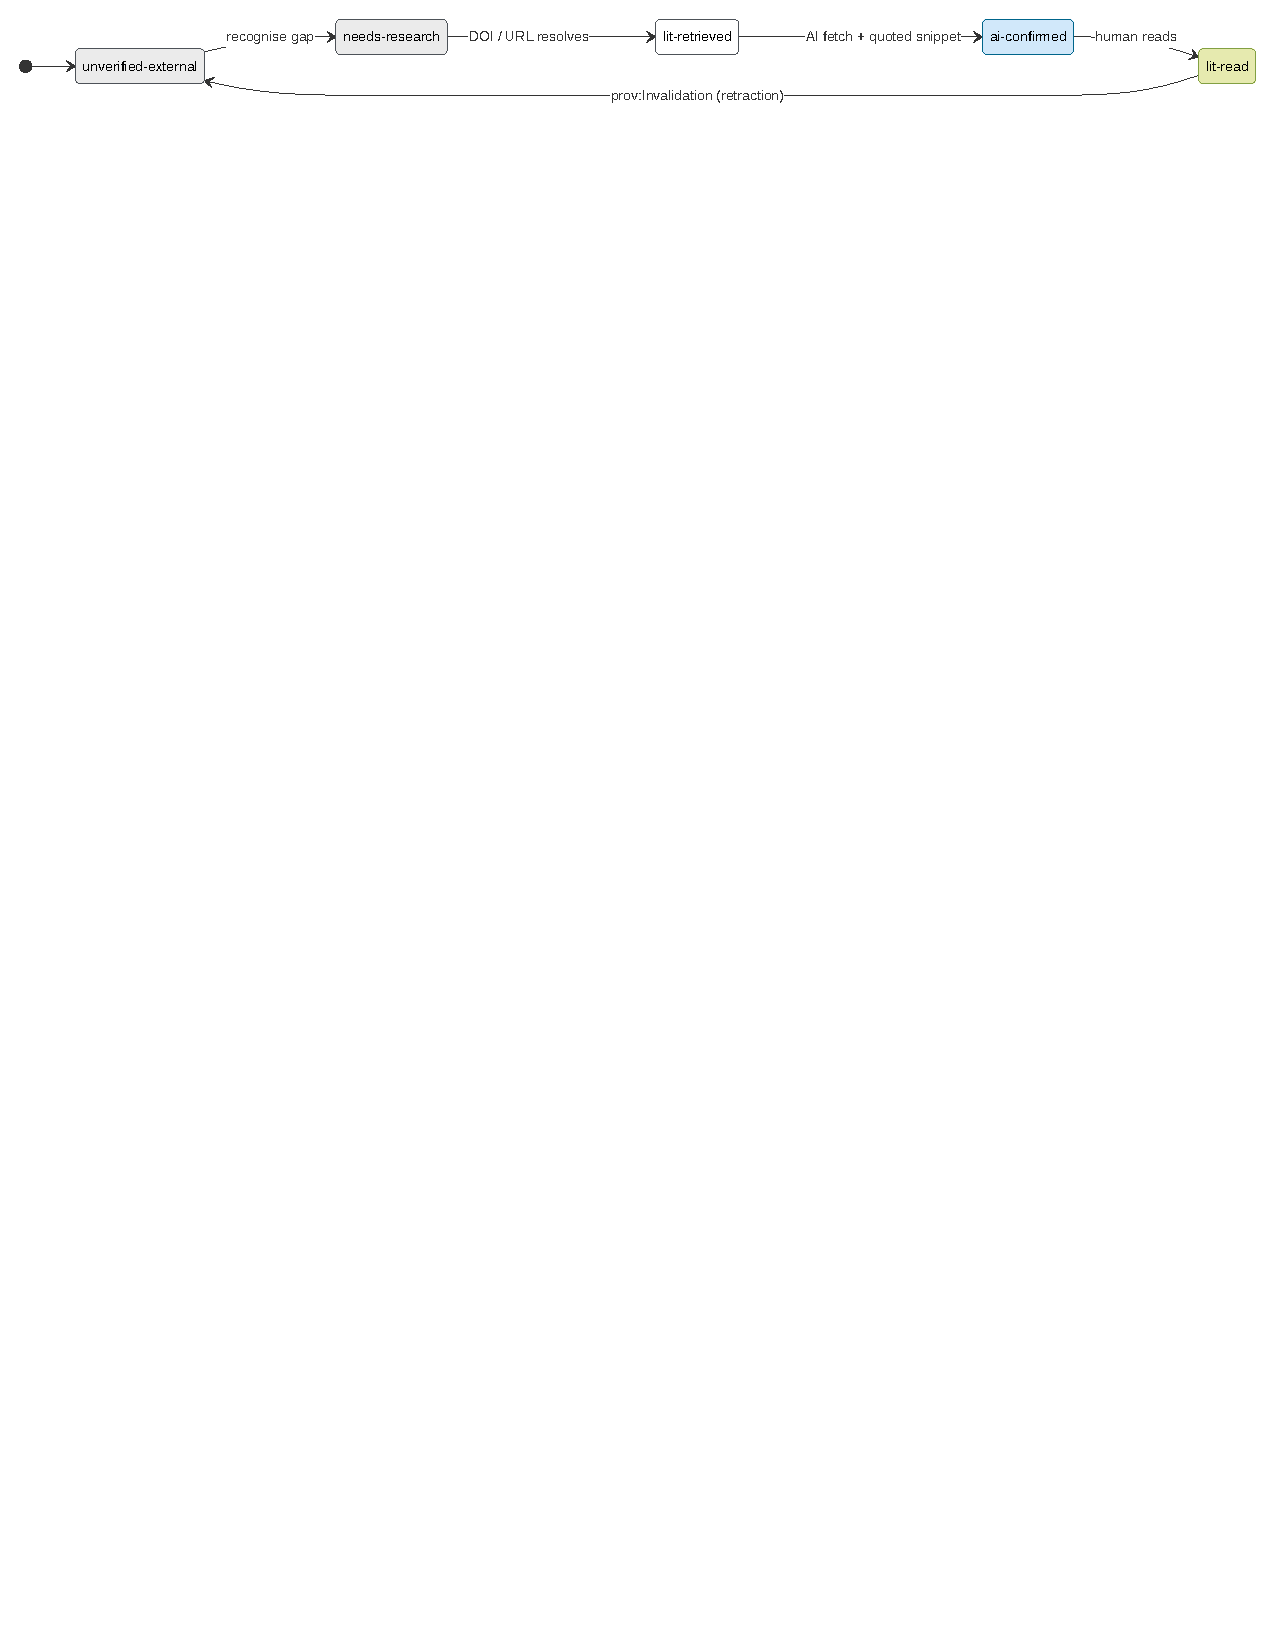
\includegraphics[width=0.92\textwidth]{../paper/figures/ladder-fsm.pdf}
  \end{center}

  \vspace{0.4em}
  \begin{itemize}
    \item \textsc{ai-confirmed} is the ceiling an LLM agent can deliver.
    \item Load-bearing claims require \textsc{lit-read}.
    \item Crosswalk: PRISMA Identification / Screening / Included;
          GRADE floor: low / moderate.
    \item Retraction is \texttt{prov:Invalidation}, never deletion
          (the only legal back-edge in the FSM).
  \end{itemize}
\end{frame}

\begin{frame}{Handback and mirror disciplines}
  \begin{block}{Handback}
    Scrutinizers never edit source. They write defect registries under
    \texttt{doc/handbacks/}. The repair is a separate commit by the prose
    owner. \emph{What did the scrutinizer flag?} has a single canonical
    answer in the git history.
  \end{block}

  \begin{block}{Mirror}
    Every primary artefact has a (source, render) pair. The build either
    agrees or fails.
  \end{block}

  \begin{block}{The invariant}
    The manuscript, the PROV-O graph, the logbook, \textbf{and the slide decks}
    are primary artefacts and must remain consistent and up to date at all times.
  \end{block}
\end{frame}

% ===================================================================
\sectiondivider{4. Eight integrated practices}
% ===================================================================

\begin{frame}{Eight practices, none novel on its own}
  \footnotesize
  \begin{tabular}{rlp{5.0cm}}
    \toprule
    \# & Practice & Failure mode \\
    \midrule
    1 & Transcript preservation              & session loss \\
    2 & Verification-status labelling (FSM)  & claim--evidence drift \\
    3 & Per-claim provenance maps            & fabricated citations \\
    4 & Mirror discipline                    & placeholder dishonesty \\
    5 & Recursive meta-process documentation & methodological-tract failure \\
    6 & Base-rate-anchored AI disclosure     & perfunctory disclosure \\
    7 & Legal honesty about authorship       & inflated co-author claims \\
    8 & FAIR alignment as \textbf{precondition} & retrofit cost \\
    \bottomrule
  \end{tabular}

  \vspace{0.6em}
  \normalsize
  \textit{The integration is the contribution.}
\end{frame}

\begin{frame}{Why eight (and not seven, or nine)}
  \begin{itemize}
    \item Each practice mitigates one or more named failure modes.
    \item Removing any one \textbf{exposes a specific failure mode that the others do not cover}.
    \item Adding a ninth (e.g. the supervisory-glance / multi-tracked-research pattern) is on the table for revision.
  \end{itemize}

  \vspace{0.4em}
  Bibliography grounded in real literature: stochastic parrots, datasheets,
  model cards, PRISMA, GRADE, ICMJE, USCO, UrhG, fabrication base rates,
  model collapse, AI-energy literature.
\end{frame}

% ===================================================================
\sectiondivider{5. Domain ontologies and the longer arc}
% ===================================================================

\begin{frame}{Extensibility through domain ontologies}
  PROV-O is the spine; it does not have to be the only ontology in the graph.

  \begin{itemize}
    \item \textbf{SOSA / SSN} (Janowicz 2019) for sensor-observation claims.
    \item \textbf{OM-2} (Rijgersberg 2013) and \textbf{QUDT} for units of measure.
    \item A \texttt{fair2r:Claim} carries \texttt{prov:wasDerivedFrom} for evidence and a domain-ontology link for value semantics.
  \end{itemize}

  \vspace{0.4em}
  Failure modes prose alone cannot reach (a value coherent in its citation but
  \textbf{wrong in its units}) become \textbf{graph queries} and SHACL shapes.

  \vspace{0.3em}
  \emph{Konkrete standardisierte Methode.}
\end{frame}

\begin{frame}{The bioinformatics precedent}
  Under data-volume pressure, bioinformatics standardised semantic tagging
  (the Gene Ontology, Ashburner 2000) so that genes, proteins, and their
  relations could be referenced unambiguously across labs.

  \begin{itemize}
    \item The ontology was \textbf{not a research output}; it was the precondition for research that scaled.
    \item The community's investment is what made the next decade possible.
  \end{itemize}

  \vspace{0.4em}
  LLM-assisted scholarship is now in an analogous moment.
\end{frame}

\begin{frame}{Future research success: three properties}
  \footnotesize
  \begin{tabular}{p{4.6cm}p{6.4cm}}
    \toprule
    Property & F(AI)\textsuperscript{2}R support \\
    \midrule
    \textbf{Provenance models} for hypothesis development & verification ladder; per-claim graph \\
    \addlinespace
    \textbf{Graph interconnectivity} across institutional knowledge graphs (Helmholtz cross-centre, fully-instrumented) & PROV-O + domain ontologies \\
    \addlinespace
    \textbf{Clever experimental validation} that uses the graph to identify the next testable deviation & recursive case study; audit pass \\
    \bottomrule
  \end{tabular}

  \vspace{0.6em}
  \normalsize
  Some standard with these properties is now load-bearing for the next decade.\\
  F(AI)\textsuperscript{2}R is one offer among several the community can refine.
\end{frame}

% ===================================================================
\sectiondivider{6. This paper, generated by this process}
% ===================================================================

\begin{frame}{Recursive attestation}
  \begin{itemize}
    \item Repository: \texttt{noheton/f-ai-r}. Public Pages site. CI-built draft PDF.
    \item Every section has a \texttt{fair2r:Section} IRI; every named claim a \texttt{fair2r:Claim} IRI.
    \item 1300+ triples in \texttt{doc/provenance.ttl}. 50 bib entries. 25-page Pages site.
    \item Reading queue auto-regenerated from the graph: 45+ entries (highest-leverage first).
    \item Replay: \texttt{git clone \dots\ \&\&\ make -C paper pdf} $\to$ identical PDF, or you found a defect.
  \end{itemize}
\end{frame}

\begin{frame}{Field notes from the second cooperative writing project}
  \begin{itemize}
    \item Researcher role shifts toward \textbf{experimentation}; humanities exception.
    \item \textbf{Prompt-craft is closer to programming than to drafting} for CS-trained researchers.
    \item Responsibility includes the rooms after publication --- conferences, panels, reviewer correspondence.
    \item \textbf{Cooperation as coupling rule.} Model on prose-craft side: accelerator. Model on abstracting side: cultural blender.
    \item Diagnostic: \emph{would the abstraction have been thinkable without the model?}
  \end{itemize}
\end{frame}

% ===================================================================
\sectiondivider{7. Failure modes and sustainability}
% ===================================================================

\begin{frame}{Eight named failure modes}
  \footnotesize
  \begin{tabular}{p{4.4cm}p{6.6cm}}
    \toprule
    Mode & Mitigation \\
    \midrule
    Fabricated citations          & verification ladder + provenance map \\
    Claim--evidence drift         & handback discipline \\
    Sloppification (drift in quotes) & mirror discipline on quotations \\
    Model collapse                & transcript preservation + disclosure \\
    List-of-lists prose           & readability scrutinizer \\
    Hedging chains                & 1 hedge per 6--8 sentences, paired with commitment \\
    Placeholder dishonesty        & asset honesty over completeness \\
    Dual use                      & made visible, not eliminated \\
    \bottomrule
  \end{tabular}

  \vspace{0.4em}
  \normalsize
  Residual: pre-publication leakage, audience fatigue, adversarial review.
\end{frame}

\begin{frame}{Sustainability is not a footnote}
  \begin{itemize}
    \item Inference burns compute (Strubell, Patterson, Luccioni, Li). Disclosure should include the order-of-magnitude inference budget.
    \item Frontier-model dependence is a \textbf{stranded-asset risk}. Receipts preserved; capability not portable.
    \item Equity: groups without frontier-model access cannot apply F(AI)\textsuperscript{2}R at the same rung.
    \item Smaller-model fallbacks for routine audit passes; an honestly-declared lower-rung distribution is preferable to a forged higher-rung one.
  \end{itemize}
\end{frame}

% ===================================================================
\sectiondivider{8. Anticipated objections}
% ===================================================================

\begin{frame}{Six objections we have heard}
  \footnotesize
  \begin{tabular}{p{5.0cm}p{6.0cm}}
    \toprule
    Objection & Response \\
    \midrule
    ``Just FAIR with extra steps.''       & Re-readings are precedent; audit pass on \textbf{R} is materially different. \\
    ``Eight practices is too expensive.'' & Eight is the minimum; dropping any one exposes a failure mode. \\
    ``Graphs add bureaucracy without preventing fraud.'' & Graphs make fraud \textbf{detectable by inspection}. \\
    ``You cannot check the model's reasoning.'' & True; we check the \textbf{output's relationship to the input}. \\
    ``This privileges well-resourced groups.'' & Real; named honestly; partial mitigations. \\
    ``Position paper should not also be worked example.'' & Practice 5 requires the recursion. \\
    \bottomrule
  \end{tabular}
\end{frame}

% ===================================================================
\sectiondivider{9. Submission and call to action}
% ===================================================================

\begin{frame}{Submission conditions (RDA / FORCE11 / HMC)}
  We will submit F(AI)\textsuperscript{2}R as a candidate community recommendation \textbf{when}:
  \begin{enumerate}
    \item Human-author consent recorded in \texttt{doc/publication-consent.md} (currently \emph{NOT YET GIVEN}).
    \item \textbf{At least one external case study} has adopted the pattern on a paper unrelated to either the source repository or this one, public under a permissive licence.
  \end{enumerate}

  \vspace{0.4em}
  The conditions are the minimum we need to distinguish a single-author idiosyncrasy from a transferable pattern.
\end{frame}

\begin{frame}{The longer arc}
  F(AI)\textsuperscript{2}R is \textbf{the entry ticket, not the destination.}

  \vspace{0.4em}
  We are \emph{not} arguing F(AI)\textsuperscript{2}R has to be \emph{the} standard.

  \vspace{0.4em}
  We are arguing that \textbf{some standard with these three properties} ---
  provenance models for hypothesis development,
  graph interconnectivity across institutional knowledge graphs,
  clever experimental validation against the graph ---
  is now load-bearing for the next decade of scholarship.
\end{frame}

% ===================================================================
% Thanks
% ===================================================================

\sectiondivider{Thank you}

\begin{frame}{}
  \textbf{Repository.} \texttt{github.com/noheton/f-ai-r}\\
  \textbf{Site.} \texttt{noheton.github.io/f-ai-r}\\
  \textbf{Draft PDF.} \texttt{github.com/noheton/f-ai-r/releases}

  \vspace{0.8em}
  \emph{The pipeline is the team; the team is the methodology.}\\
  \emph{Specialisation reduces hallucination at the seam.}\\
  \emph{Naming what we are already doing is the first step toward surrendering it to peer scrutiny.}

  \vspace{0.8em}
  Questions and discussion welcome.
\end{frame}

% ===================================================================
\sectiondivider{Backup}
% ===================================================================

\begin{frame}{F(AI)\textsuperscript{2}R cell mapping (selected)}
  \footnotesize
  \begin{tabular}{p{2.2cm}p{4.4cm}p{4.4cm}}
    \toprule
    Sub-principle & Authoring (AI\textsubscript{1}) & Audit (AI\textsubscript{2}) \\
    \midrule
    F1 (identifier)        & Zenodo DOI; per-claim IRIs                 & metadata surfaces agree; IRIs unique \\
    A1 (retrievable)       & public Git; static site                     & clone-and-build on clean machine \\
    I1 (formal language)   & Turtle for provenance; \LaTeX{} for prose   & validate Turtle; lint CFF \\
    I2 (FAIR vocab)        & PROV-O + DCTERMS + FOAF + \texttt{fair2r:}  & namespaces stable \\
    R1.2 (provenance)      & the provenance graph itself                  & replay; report drift \\
    \bottomrule
  \end{tabular}
\end{frame}

\begin{frame}{Verification ladder budget (auto-generated at build)}
  At build-time, \texttt{scripts/provenance\_analysis.py} regenerates a rung-distribution table from \texttt{doc/provenance.ttl}.

  \vspace{0.4em}
  \begin{center}
    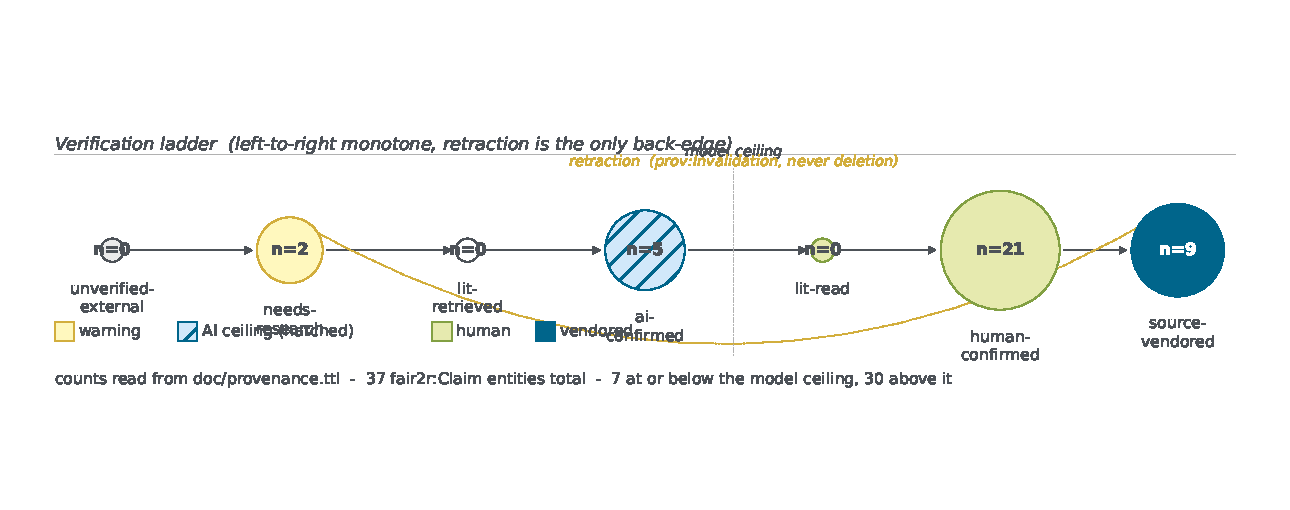
\includegraphics[width=0.96\textwidth]{../paper/figures/ladder-populations.pdf}
  \end{center}

  \vspace{0.2em}
  Sources are graded independently. Reading queue (\texttt{doc/reading-queue.md}) lists sources still at \texttt{lit-retrieved}, sorted by load-bearing weight.
\end{frame}

\begin{frame}{Imprint}
  \textbf{Florian Krebs} \quad ORCID \href{https://orcid.org/0000-0001-6033-801X}{0000-0001-6033-801X}\\
  \texttt{florian.krebs@dlr.de}

  \vspace{0.4em}
  DLR Zentrum f\"ur Leichtbauproduktionstechnologie (ZLP), Augsburg

  \vspace{0.4em}
  Helmholtz-Gemeinschaft \textperiodcentered{} NFDI4Ing \textperiodcentered{} HMC

  \vspace{0.6em}
  \textbf{Repository:} \texttt{github.com/noheton/f-ai-r}\\
  \textbf{Site:} \texttt{noheton.github.io/f-ai-r}

  \vspace{0.4em}
  \footnotesize
  Code: MIT \textperiodcentered{} Prose: CC-BY-4.0 \textperiodcentered{}
  Photo credit (where present): DLR (CC BY-NC-ND 3.0) sofern nicht anders angegeben.
\end{frame}

\end{document}
